\documentclass[handout]{beamer}

\usetheme[progressbar=frametitle]{metropolis}
\metroset{block=fill}

\subtitle{NTIN071 Automata and Grammars}
\author{Jakub Bulín (KTIML MFF UK)}

\date{Spring 2025\\ 
    \vspace{1in} 
    \begin{flushleft}
        \it \footnotesize * Adapted from the Czech-lecture slides by Marta Vomlelová with gratitude. The translation, some modifications, and all errors are mine.
    \end{flushleft}
}

%% packages

\usepackage{amsmath}
\usepackage{amssymb}
\usepackage{amsthm}
\usepackage{cancel}
\usepackage{color}
\usepackage{colortbl}
\usepackage{forest}
\usepackage[utf8x]{inputenc}
\usepackage{multicol}
\usepackage{multirow}

%% colors
\definecolor{Gray}{gray}{0.9}

%% TikZ
\usepackage{tikz}
    \usetikzlibrary{
        automata,
        arrows,
        backgrounds,
        decorations.pathmorphing,
        fit,
        positioning,
        shapes,
        shapes.geometric,
        tikzmark
    } 
    \tikzset{>=stealth',shorten >=1pt,auto,node distance=2cm}
    \tikzset{initial text={}}
    \tikzset{elliptic state/.style={draw,ellipse}}

%% amsthm
\theoremstyle{plain}
    \newtheorem*{algorithm}{Algorithm}    
    \newtheorem*{observation}{Observation}
    \newtheorem*{proposition}{Proposition}

\theoremstyle{remark}
    \newtheorem*{exercise}{Exercise}
    \newtheorem*{remark}{Remark}

%% macros
\DeclareMathOperator{\RegE}{RegE}
\DeclareMathOperator{\RL}{RL}

% Just for Lecture 2
\newcommand{\x}{$\times$}
\newcommand{\nx}{\ }



\title{Lecture 12 -- Undecidable problems, Post's correspondence problem}


\begin{document}


\frame{\titlepage}


\begin{frame}{Recap of Lecture 11}
	
    \begin{itemize}        
        \item Recursively enumerable languages are exactly those generated by (Type 0) grammars
        \begin{itemize}
            \item TM to G: simulate moves on a reversed non-terminal copy of $\omega$, generate sufficient space, cleanup if accepting state
            \item G to TM: generate all strings, check if any of them represents a valid derivation of $\omega$ (sentential forms separated by $\#$)
        \end{itemize}   
        \item Context-sensitive languages:
        \begin{itemize}
            \item context-sensitive grammars are equivalent to monotone grammars
            \item Linear Bounded Automaton (LBA): nondeterministic TM with tape limited to the length of input
            \item constructions: monotone grammar to LBA, LBA to monotone grammar
        \end{itemize}
        \item Intro to computability: an overview
        \item decision problem $\leftrightsquigarrow$ the language of all `YES' instances
        \item machine-readable encoding of TMs
    \end{itemize}
	
\end{frame}



\begin{frame}{The Diagonal language}
    
    Let \alert{$\mathrm{decode}(w)$} be the TM $M$ such that $\mathrm{code}(M)=w$. (Recall: if $w$ is not a valid code, then $\mathrm{decode}(w)$ is a fixed one-state TM with no instructions.) Then:
    $$
    \alert{L_D}=\{w\mid w\notin L(\mathrm{decode}(w))\}
    $$
        
    \begin{theorem}
        $L_D$ is not recursively enumerable.
    \end{theorem}
    
    \textbf{Proof idea:} there cannot exist a TM recognizing $L_D$: running it on its own code would lead to Barber's paradox

    \bigskip

    \begin{quote}
        ``The program accepts all programs that don't accept themselves. Does the program accept itself?''
    \end{quote}

\end{frame}


\begin{frame}{Proof that $L_D=\{w\mid w\notin L(\mathrm{decode}(w))\}$ is not RE}

    \textbf{Proof:} Assume for contradiction that $L_D=L(M)$ for some $M$. Let $w=\mathrm{code}(M)$. Then $L_D=\{w\mid w\notin L(M)\}$. Is $w\in L(M)$?
    $$
    w\in L(M)\ \Leftrightarrow\ w\in L_D\ \Leftrightarrow\ w\notin L(M)
    $$
    
    \vspace{-24pt}
    \hfill\qedsymbol

    Why `diagonal'? A variant of Cantor's diagonal argument. Order all TMs by  $M_i=\mathrm{decode}(w_i)$. Does $M_i$ accept $w_j$?

    \vspace{-12pt}
    \begin{center}
        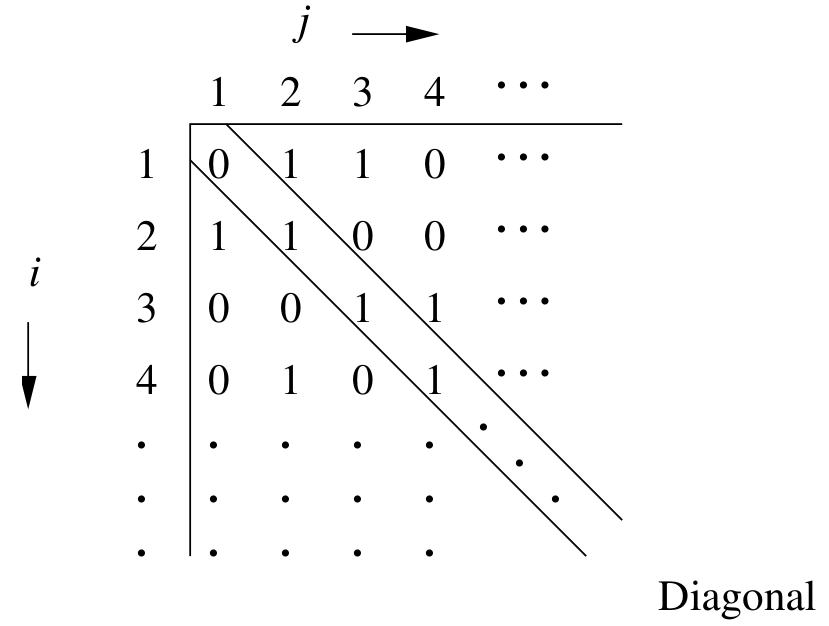
\includegraphics[width=0.48\textwidth]{files/diagonal.PNG}
    \end{center}
    \vspace{-15pt}
    A TM for $L_D$ would be one of the rows but differs from each row in the diagonal element. (Same as the proof that $\mathbb R$ is uncountable.)  
    
\end{frame}


\begin{frame}{The Universal Turing Machine}

    

\end{frame}



\begin{frame}{Summary of Lecture 12}

    \begin{itemize}
        \item the Diagonal language $L_D$ is not recursively enumerable
        \item the Universal language $L_U$, the Universal TM: simulate any $M$ on any $w$
        \item Post's theorem: $L$ recursive iff both $L,\overline{L}$ are RE
        \item $L_U$, $\overline{L_D}$ are recursively enumerable but not recursive
    \end{itemize}

\end{frame}


\end{document}